\chapter{Implementasi dan Pengujian}
\label{chap:implementasi}

Pada bab ini terdapat dua bagian, yaitu Implementasi Perangkat Lunak dan Pengujian Perangkat Lunak. Bagian implementasi akan menjelaskan tentang lingkungan pengembangan perangkat lunak dan hasil implementasi. Bagian pengujian akan berisi hasil pengujian fungsional terhadap perangkat lunak yang telah dibangun.

\section{Implementasi}
\label{sec:implementasi}

\subsection{Implementasi}
Implementasi dilakukan dengan menggunakan laptop dengan spesifikasi sebagai berikut :
\begin{enumerate}
	\item \textit{Processor} : Intel(R) Core(TM) i5-4200U CPU @ 1.60GHz 2.30GHz
	\item RAM : 4.00 GB
	\item Sistem Operasi : Windows 10 Pro 64-bit
	\item Versi Netbeans : 8.0.2
\end{enumerate}

\subsection{Hasil Implementasi}
\begin{enumerate}
	\item Tampilan Bobot Ketetanggaan
	
	
	Seperti yang telah dijelaskan pada bab \ref{chap:perancangan}, tampilan ini berfungsi untuk mengisi atribut dari masing-masing wirausaha. \textit{User} dapat memilih atribut mana yang akan dijadikan sebagai ketetanggaan dari masing-masing wirausaha dengan cara men-\textit{checklist checkbox} atribut yang diinginkan. (Gambar \ref{fig:tampilanBobot1})
	
	
	\begin{figure} [H]
	\centering  
	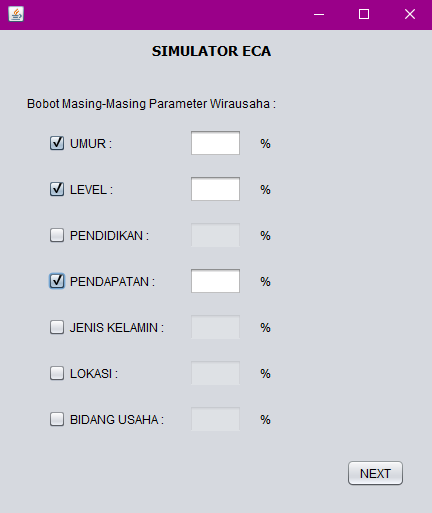
\includegraphics[width=12cm, height=13cm]{tampilanImplementasiBobot} 
		\caption[Gambar TampilanBobotKetetanggaan]{Gambar TampilanBobotKetetanggaan pada saat men-\textit{checklist checkbox}}
	\label{fig:tampilanBobot1} 
\end{figure}

	Pada saat \textit{user} sudah melakukan \textit{check list} pada \textit{checkbox}, \textit{user} harus mengisi bobot untuk setiap atribut yang telah dipilih. Total bobot atribut harus 100\%. (Gambar \ref{fig:tampilanBobot2})
	
	
	\begin{figure} [H]
	\centering  
	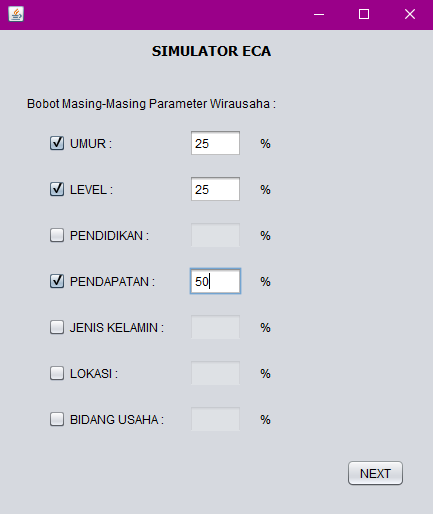
\includegraphics[width=12cm, height=13cm]{tampilanImplementasiBobot1} 
		\caption[Gambar TampilanBobotKetetanggaan]{Gambar TampilanBobotKetetanggaan pada saat mengisi bobot masing-masing atribut}
	\label{fig:tampilanBobot2} 
\end{figure}

	\item TampilanKondisiKetetanggaan
	
	Pada tampilan ini, \textit{user} diminta untuk mengisi relasi ketetanggaan pada atribut yang telah dipilih sebelumnya. (Gambar \ref{fig:tampilantetangga})
	
	\begin{figure} [H]
	\centering  
	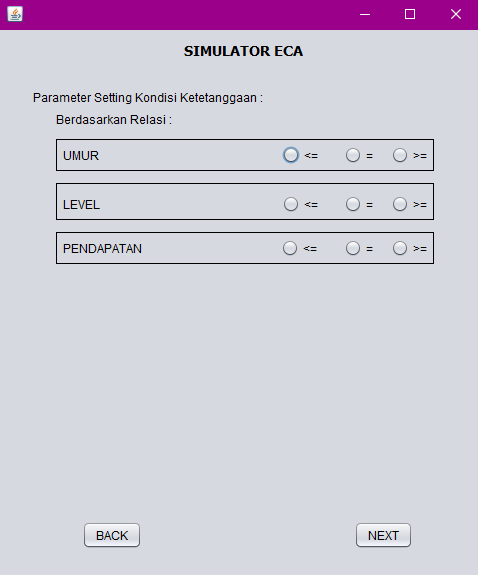
\includegraphics[width=10cm, height=12cm]{tampilanImplementasiKetetanggaan} 
		\caption[Gambar TampilanKondisiKetetanggaan]{Gambar TampilanKondisiKetetanggaan untuk atribut yang telah dipilih sebelumnya.}
	\label{fig:tampilantetangga} 
\end{figure}

	\textit{User} dapat mengisi relasi melalui \textit{radio button} dan \textit{user} hanya bisa memilih salah satu diantara tiga relasi tersebut. (Gambar \ref{fig:tampilantetangga1})
	
	\begin{figure} [H]
	\centering  
	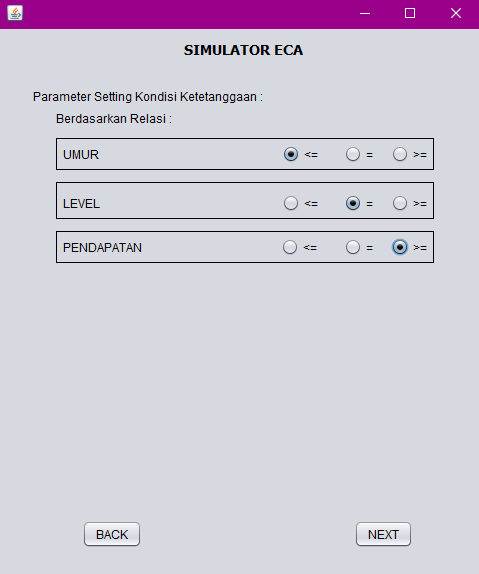
\includegraphics[width=10cm, height=12cm]{tampilanImplementasiKetetanggaan1} 
		\caption[Gambar TampilanKetetanggaan]{Gambar TampilanKondisiKetetanggaan pada saat mengisi relasi ketetanggaan}
	\label{fig:tampilantetangga1} 
\end{figure}

	\item TampilanKondisiEksternal
	
	Pada tampilan ini, \textit{user} akan mengisi bobot masing-masing faktor publik. Jumlah dari seluruh bobot harus 100\%. (Gambar \ref{fig:tampilaneksternal1})
	
		\begin{figure} [H]
	\centering  
	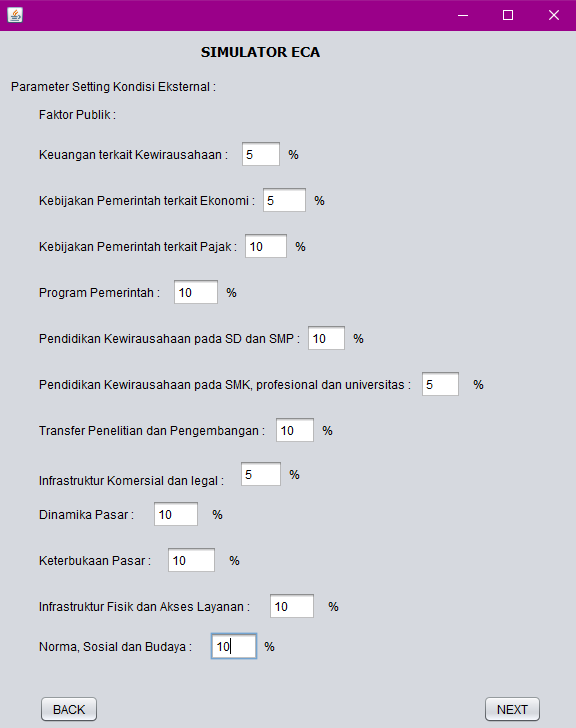
\includegraphics[width=10cm, height=12cm]{tampilanImplementasiEksternal} 
		\caption[Gambar TampilanKetetanggaan]{Gambar TampilanKondisiEksternal pada saat mengisi bobot faktor publik}
	\label{fig:tampilaneksternal1} 
\end{figure}

	\item TampilanDataWirausaha
	
 	Pada tampilan data wirausaha \textit{user} dapat meng-klik \textit{button} "OPEN FILE" yang fungsinya untuk membuka file data wirausaha yang akan disimulasikan. Data wirausaha berisi jenis kelamin, umur, usia bisnis, kategori usaha, subkategori usaha, pendidikan, lokasi, pendapatan, level dan point. Point merupakan hasil perhitungan masing-masing wirausaha pada kondisi internal. (Gambar \ref{fig:tampilandata})
	
		\begin{figure} [H]
	\centering  
	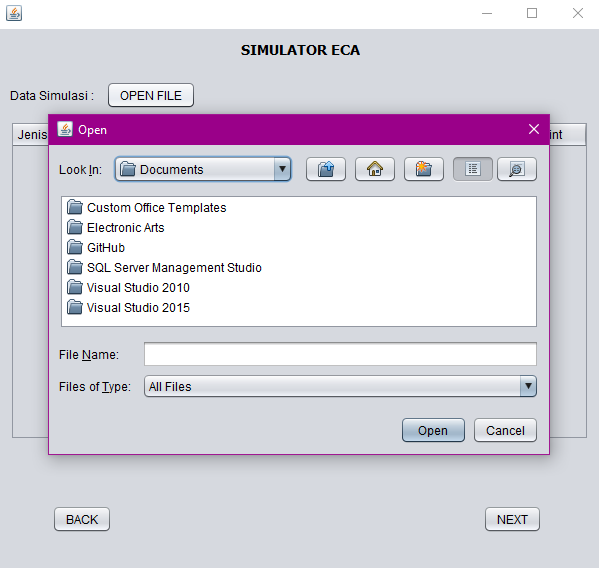
\includegraphics[width=12cm, height=12cm]{tampilanImplementasiData} 
		\caption[Gambar TampilanDataWirausaha]{Gambar TampilanDataWirausaha pada saat membuka \textit{button} "OPEN FILE"}
	\label{fig:tampilandata} 
\end{figure}

Berikut merupakan tampilan data wirausaha yang telah dipilih oleh \textit{user}. (Gambar \ref{fig:tampilandata1})
	
		\begin{figure} [H]
	\centering  
	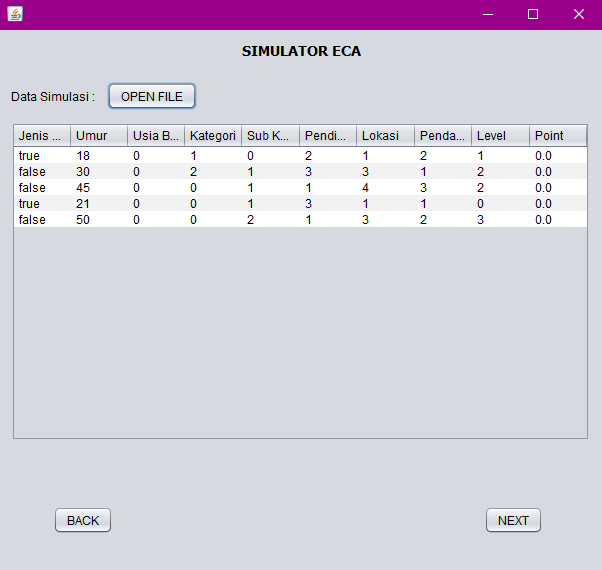
\includegraphics[width=12cm, height=12cm]{tampilanImplementasiData1} 
		\caption[Gambar TampilanDataWirausaha]{Gambar TampilanDataWirausaha saat menampilkan isi dari file}
	\label{fig:tampilandata1} 
\end{figure}

	\item TampilanSimulasi
	
	Pada tampilan ini \textit{user} diminta untuk mengisi bobot dari a,b,c,threshold dan periode. Total nilai dari a,b dan c harus 1. Setelah mengisi masing-masing nilai, \textit{user} dapat melakukan simulasi dengan cara meng-klik \textit{button} "SIMULATE".(Gambar \ref{fig:tampilansimulasi})
	
		\begin{figure} [H]
	\centering  
	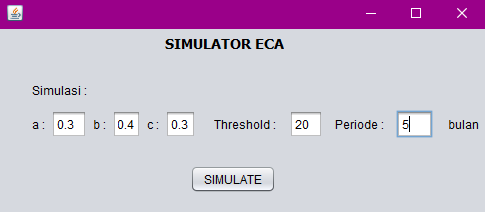
\includegraphics[width=14cm, height=8cm]{tampilanImplementasiSimulasi1} 
		\caption[Gambar TampilanSimulasi]{Gambar TampilanSimulasi pada saat mengisi bobot a,b,c,threshold dan periode}
	\label{fig:tampilansimulasi} 
\end{figure}

	\item TampilanHasil
\end{enumerate}